\documentclass{article}
\usepackage[english]{babel}
\usepackage{amsmath}
\usepackage{graphicx}
\usepackage{listings}

\begin{document}
\begin{titlepage}
  \begin{center}
    \vspace*{1cm}
    
    \Huge
    \textbf{Matrix Multiplication}
    
    \vspace{0.5cm}
    \LARGE
    PROJECT 2
    
    \vspace{1.5cm}
    
    \textbf{Feiyang Zheng}
    
    \vfill
    
    \vspace{0.8cm}
    
    \Large
    Department of Mathematics\\
    SUSTech\\
    China\\{March 2024}
    
  \end{center}
\end{titlepage}

\section{Introduction}

Matrix multiplication is a fundamental operation in linear algebra. In this project, we will implement a matrix multiplication algorithm in C and Java, then compare their performances with different matrix sizes and different optimization levels. Two different matrix multiplication algorithms are implemented in C and Java. The first algorithm is the naive matrix multiplication algorithm, which has a time complexity of $O(n^3)$. However, during the testing, the naive matrix multiplication algorithm is found to have a time complexity larger than $O(n^3)$. After some test with different matrix sizes, the author purpose that such behavior is due to the cache miss. The naive matrix multiplication algorithm is implemented in both C and Java.

\section{Naive Matrix Multiplication}
\subsection{Algorithm}

The code for naive matrix multiplication is as follows:
\begin{verbatim}
void multiply(float* a, float* b, float* result, int n) {
  for (int i = 0; i < n; i++) {
    for (int j = 0; j < n; j++) {
      for (int k = 0; k < n; k++)
        result[i*n + j] += a[i*n + k] * b[k*n + j];
    }
}
}
\end{verbatim}

Instead of using \texttt{float \* \*} 2D array, 1D array is implemented because Prof. Yu claims on C programming class that this can reduce the number of jumping, which we will verify in the later part of the report.

\subsection{Comparison between C and Java}
To make sure that both both C and Java are running the same algorithm, the same matrix size and the same random numbers are used in both C and Java. because the pseudo-random number generator is different in C and Java, in order to have exact same matrices for multiplication, the Java program is designed to read hexadecimal float from a txt that is generated by the C program. 

\subsection{Performance}
For the underlying algorithm, four different compilation flags are used to compile the C code, which are \texttt{-O0}, \texttt{-O1}, \texttt{-O2}, \texttt{-O3} and \texttt{-Ofast}. The Java code is compiled with the default optimization level. The matrix sizes are \(n=(2^i)^2,\quad i=\{1,2,\cdots,10\}\). The time is measured using the \texttt{clock()} function in C and the \texttt{System.currentTimeMillis()} function in Java. The time is measured 100 times, and the average time is calculated. The results are shown in figure \ref{fig:naive}.

\begin{figure}[htbp]
  \centering
  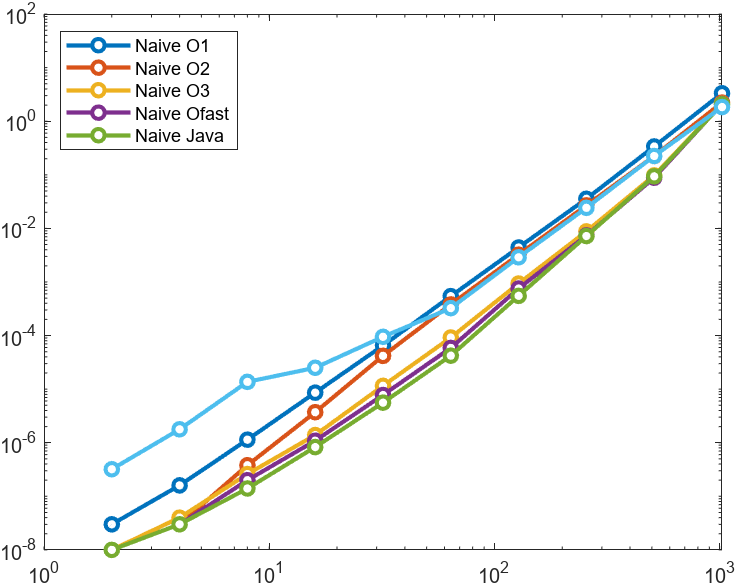
\includegraphics[width=0.8\textwidth]{figure/naive.png}
  \caption{The logrithm plot of the matrix size \(n\) versus the mean time \(t\).} \label{fig:naive}
\end{figure}


from the figure \ref{fig:naive}, we could see that \texttt{O2}, \texttt{O3}, and \texttt{Ofast} seem to form convex curves. In theory, these curves should be a straight line whose slope is approximately 3. What's more, the time cumsumption for \(n=1024\) increases dramatically comparing to \(n=512\), such phenomenon is observed in all C programs. all four programs takes around the same amount of time regardless of their compilation flags. Even Java was able to run faster than them by 10\%. Take \texttt{Ofast} as an example, in the table we could observe that the runtime increases by more than 20 times when scaling up from 512 to 1024, while in theory, the runtime from \(n\) to \(2n\) should be only 8 times larger.
\begin{table}[htbp]
  \centering
  \begin{tabular}{lllll}
  n    & t   & runtime(sec)    &  &  \\
  \hline
  2    & 100 & 0.000001   &  &  \\
  4    & 100 & 0.000003   &  &  \\
  8    & 100 & 0.000014   &  &  \\
  16   & 100 & 0.000083   &  &  \\
  32   & 100 & 0.000560   &  &  \\
  64   & 100 & 0.004216   &  &  \\
  128  & 100 & 0.055142   &  &  \\
  256  & 100 & 0.719766   &  &  \\
  512  & 100 & 9.369874   &  &  \\
  1024 & 100 & 207.351453 &  & 
  \end{tabular}
\end{table}

After consulting my roommate, whom is a former OIer, he suggests that such behavior is propably caused by the threshold CPU reading memory to its cache. Furthermore, he suggests that I should try block multiplication, which has the same time complexity \(O(n^3)\) while minimizing the throughput between CPU and memory.

\section{Block Matrix Multiplication}

\subsection{Algorithm}

The code of block matrix multiplication works as follows:

\begin{verbatim}
  void block_multiply(float* a,float* b,float* result,int n,int block_size) 
  {
    for (int i = 0; i < n; i += block_size) {
      for (int j = 0; j < n; j += block_size) {
        for (int k = 0; k < n; k += block_size) {
          for (int ii = i; ii < i + block_size; ii++) {
            for (int jj = j; jj < j + block_size; jj++) {
              for (int kk = k; kk < k + block_size; kk++) {
                result[ii*n+jj] += a[ii*n+kk] * b[kk*n+jj];
              }
            }
          }
        }
      }
    }
  }
\end{verbatim}

The block multiply function assumes that the size of the matrices \(n\) is a multiple of the block size. It breaks the input matrices into smaller sub-matrices or blocks, and then performs the multiplication on these smaller blocks. This can be more efficient on modern hardware because it can take better advantage of the CPU cache.

\subsection{Performance}

Substituting the new algorithm into the programs and rerun the test aforementioned. We can retrieve the result in figure \ref{fig:block}.

\begin{figure}[htbp]
  \centering
  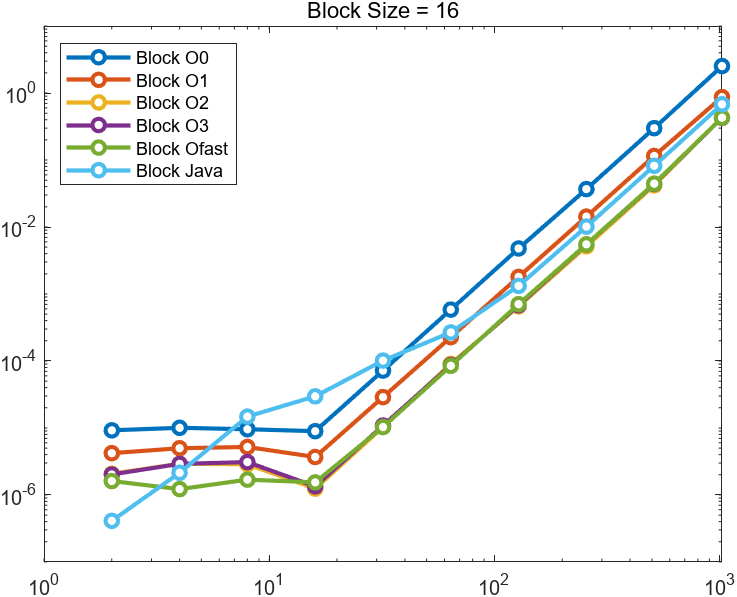
\includegraphics[width=0.8\textwidth]{figure/block.png}
  \caption{The logrithm plot of the matrix size \(n\) versus the mean time \(t\).} \label{fig:block}
\end{figure}

From figure \ref{fig:block} we can observe that the time cumsumption is linear as the matrix size scales up when the matrix size is larger than 16, the block size. What's more, we notice that the runtime of matrix multiplication is almost identical with flags \texttt{O2}, \texttt{O3}, and \texttt{Ofast}. The runtime of Java lies between \texttt{O1} and \texttt{O2}. The runtime of \texttt{O0} is the largest among all. The runtime of \texttt{O1} is 2 times larger than \texttt{Ofast} when \(n=1024\). The runtime of Java is 1.5 times larger than \texttt{Ofast} when \(n=1024\). However, if we use \texttt{ls -l} command to check the size of the executable file, we can see that the size of the executable file of \texttt{O1} is 20720; \texttt{O1}, \texttt{O2} and \texttt{O3} are all 16656 bytes, while the size of the executable file of \texttt{Ofast} is 18168 bytes. Despite having a larger binary executable, the \texttt{Ofast} fails to out compete the other two in this case.


\begin{table}[htbp]
  \centering
  \begin{tabular}{lllll}
    Flag & Naive & Block \\
    \hline
    O0    & 20720 & 20720 \\
    O1    & 16656 & 16656 \\
    O2    & 16656 & 16656 \\
    O3    & 16656 & 16704 \\
    Ofast & 18168 & 22304
  \end{tabular}
  \caption{The size of the executable file of the C program in bytes.}
\end{table}

Besides, the performance of the block matrix multiplication algorithm is better than the naive matrix multiplication algorithm. The time consumption of the block matrix multiplication algorithm is about 1/3 of the naive matrix multiplication algorithm when the matrix size is 1024. The block matrix multiplication algorithm is more efficient than the naive matrix multiplication algorithm because it can take better advantage of the CPU cache.

\subsection{Block Size}

The block size is a parameter that can be tuned to optimize the performance of the block matrix multiplication algorithm. The block size should be chosen based on the size of the CPU. In the following, we will test the performance of the block matrix multiplication algorithm with different block sizes. The matrix size is \(n=1024\), and the block size is \(b=\{1,2,4,8,16,32,64,128,256\}\). The results are shown in figure \ref{fig:blocksize}.

\begin{figure}[htbp]
  \centering
  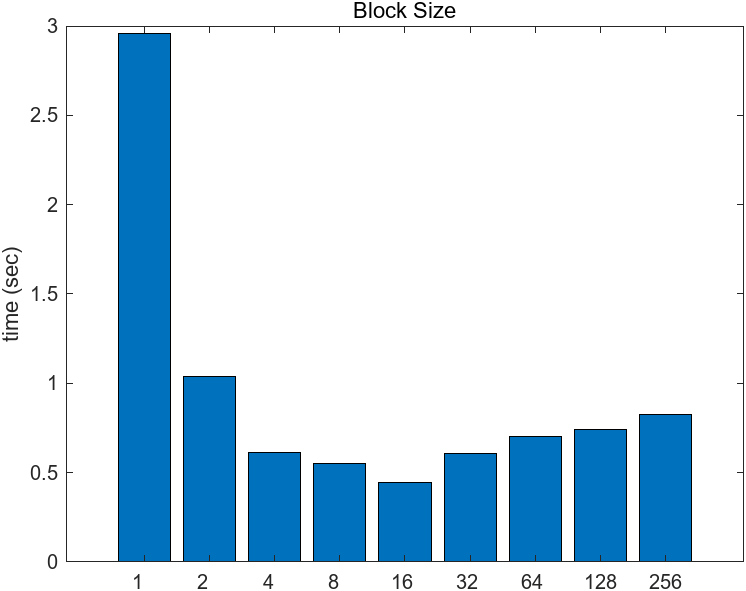
\includegraphics[width=0.8\textwidth]{figure/blocksize.png}
  \caption{The logrithm plot of the block size \(b\) versus the mean time \(t\).} \label{fig:blocksize}
\end{figure}

from the experiment, we can see that the block size of 16 is the best choice for the block matrix multiplication algorithm. The time consumption is the smallest when the block size is 16. 

\section{Arch Native}
Besides compilation flags, the author also tried to use \texttt{-march=native} to compile the C program. \texttt{-O3} is enabled in both test and the matrix size is set to 1024. The performance is shown in figure \ref{fig:march}.
\begin{figure}[htbp]
  \centering
  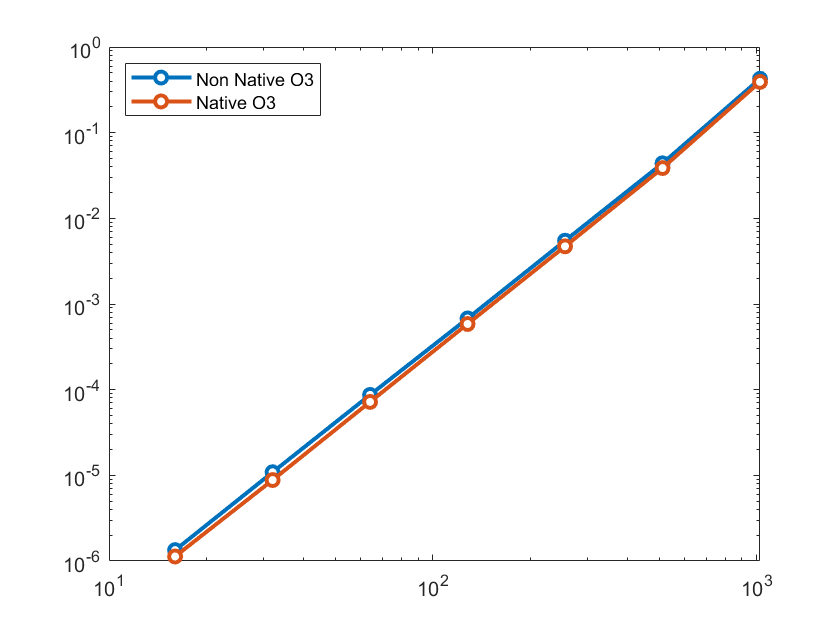
\includegraphics[width=0.8\textwidth]{figure/march.png}
  \caption{The logrithm plot of the matrix size \(n\) versus the mean time \(t\).} \label{fig:march}
\end{figure}

From figure \ref{fig:march}, we can see that the performance of \texttt{-march=native} is almost identical to the performance of \texttt{O3}, but still slightly better than non native compilation. The performance of \texttt{-march=native} is better than the performance of \texttt{O3} because the compiler can generate code that is optimized for the specific CPU architecture at the expense of portability.

\newpage
\section{2D Array vs 1D Array}
\texttt{malloc} for 2D array is slightly tricky. The code for 2D array is as follows:
\begin{verbatim}
float (*a)[n] = malloc(sizeof(float[n][n]));
\end{verbatim}

The code for 1D array is as follows:
\begin{verbatim}
float* a = malloc(n*n*sizeof(float));
\end{verbatim}

for matrix multiplication, the 2D array implementation is as follows:
\begin{verbatim}
void block_multiply(int n, float a[n][n], float b[n][n],
 float result[n][n], int block_size) {
  for (int i = 0; i < n; i += block_size) {
    for (int j = 0; j < n; j += block_size) {
      for (int k = 0; k < n; k += block_size) {
        for (int ii = i; ii < i + block_size; ii++) {
          for (int jj = j; jj < j + block_size; jj++) {
            for (int kk = k; kk < k + block_size; kk++) {
              result[ii][jj] += a[ii][kk] * b[kk][jj];
            }
          }
        }
      }
    }
  }
}
\end{verbatim}
The rest of the code is the same as the 1D array implementation. The performance of the 2D array implementation is shown in figure \ref{fig:2d}. Only flag \texttt{O3} is used in this experiment.
\begin{figure}[htbp]
  \centering
  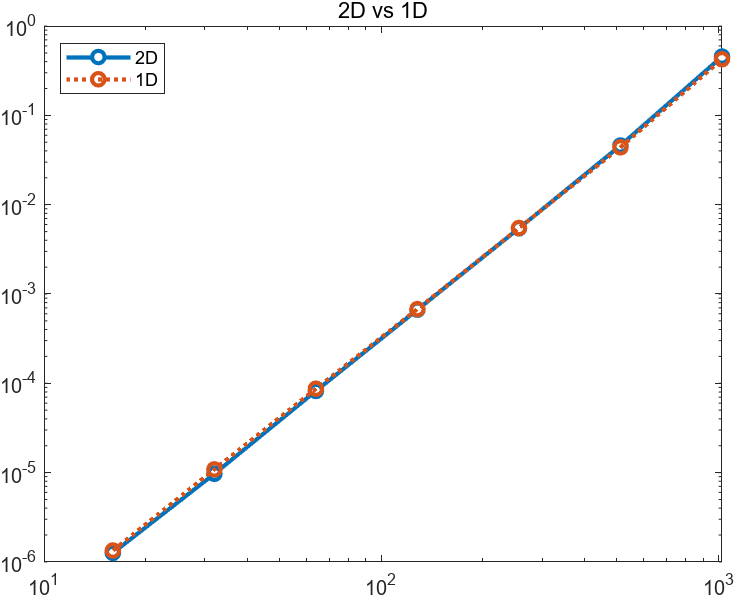
\includegraphics[width=0.8\textwidth]{figure/2d.png}
  \caption{The logrithm plot of the matrix size \(n\) versus the mean time \(t\).} \label{fig:2d}
\end{figure}

From figure \ref{fig:2d}, we can see that the performance of the 2D array implementation is almost identical to the 1D array implementation. This might because the gcc compiler optimizes the 2D array implementation to be the same as the 1D array implementation. The 2D array implementation is easier to understand and write, so it is recommended to use the 2D array implementation.


\section{Conclusion}
From the above experiments, we can conclude that the block matrix multiplication algorithm is more efficient than the naive matrix multiplication algorithm. The block matrix multiplication algorithm can take better advantage of the CPU cache. The block size of 16 is the best choice for the block matrix multiplication algorithm. The performance of the \texttt{-march=native} flag is almost identical to the performance of the \texttt{O3} flag, but still slightly better than non native compilation. The 2D array implementation is almost identical to the 1D array implementation. The 2D array implementation is easier to understand and write, so it is recommended to use the 2D array implementation. 

\section{Appendix}
Testing bash scripts for C are as follows:
\begin{verbatim}
for flag in {1,2,3,"fast"}; do
  echo "flag="$flag
  gcc -o ./bin/block/matmul_O$flag matmul.c -O$flag -lm
  echo "n,t,runtime" > data/block/matmul_O$flag.csv
  n=2
  t=100
  while [ $n -le 1024 ]; do
    echo "n=$n"
    output=$(./bin/block/matmul_O$flag -n $n -t $t -b 16)
    runtime=$(echo "$output" | grep -oP 'Time spent: \K[0-9.]+')
    echo "$n,$t,$runtime" >> data/block/matmul_O$flag.csv
    n=$((n * 2))
  done
done
\end{verbatim}

Testing bash scripts for Java are as follows:
\begin{verbatim}
gcc -o ./bin/block/matmul_O3 matmul.c -Ofast -lm
javac MatrixMultiplication.java
echo "n,t,runtime" > data/block/matmul_Java.csv
n=2
t=100
while [ $n -le 1024 ]; do
  echo "n=$n"
  ./bin/block/matmul_O3 -n $n // generate matrix.txt
  output=$(java MatrixMultiplication $n $t 16)
  runtime=$(echo "$output" | grep -oP 'Time spent: \K[0-9.]+')
  echo "$n,$t,$runtime" >> data/block/matmul_Java.csv
  n=$((n * 2))
done
\end{verbatim}

Data of runtime for C and Java are as follows:
\begin{verbatim}
  naive_O0 = [2,100,0.000003;
  4,100,0.000016;
  8,100,0.000114;
  16,100,0.000860;
  32,100,0.006508;
  64,100,0.054426;
  128,100,0.441053;
  256,100,3.572119;
  512,100,33.793496;
  1024,100,332.757244];
naive_O1 = [2,100,0.000001;
  4,100,0.000003;
  8,100,0.000038;
  16,100,0.000371;
  32,100,0.004181;
  64,100,0.038126;
  128,100,0.323326;
  256,100,2.691324;
  512,100,22.420946;
  1024,100,222.942437];

naive_O2 = [2,100,0.000001;
  4,100,0.000004;
  8,100,0.000026;
  16,100,0.000139;
  32,100,0.001154;
  64,100,0.009184;
  128,100,0.093540;
  256,100,0.878346;
  512,100,9.752917;
  1024,100,212.622344];

naive_O3 = [2,100,0.000001;
  4,100,0.000003;
  8,100,0.000020;
  16,100,0.000109;
  32,100,0.000777;
  64,100,0.005882;
  128,100,0.075544;
  256,100,0.740258;
  512,100,8.837067;
  1024,100,209.681480];

naive_Ofast = [2,100,0.000001;
  4,100,0.000003;
  8,100,0.000014;
  16,100,0.000083;
  32,100,0.000560;
  64,100,0.004216;
  128,100,0.055142;
  256,100,0.719766;
  512,100,9.369874;
  1024,100,207.351453];

naive_Java = [2,100,0.000032;
  4,100,0.000178;
  8,100,0.001368;
  16,100,0.002507;
  32,100,0.009477;
  64,100,0.032536;
  128,100,0.288704;
  256,100,2.423865;
  512,100,22.469949;
  1024,100,183.820344];

  block_O0 = [2,100,0.000921;
  4,100,0.001005;
  8,100,0.000956;
  16,100,0.000895;
  32,100,0.007181;
  64,100,0.058476;
  128,100,0.478340;
  256,100,3.680024;
  512,100,29.897884;
  1024,100,252.758559];

block_O1 = [2,100,0.000420;
  4,100,0.000498;
  8,100,0.000520;
  16,100,0.000368;
  32,100,0.002884;
  64,100,0.022633;
  128,100,0.180047;
  256,100,1.429043;
  512,100,11.506494;
  1024,100,86.933194];

block_O2 = [2,100,0.000207;
  4,100,0.000292;
  8,100,0.000287;
  16,100,0.000124;
  32,100,0.001031;
  64,100,0.009053;
  128,100,0.065344;
  256,100,0.513909;
  512,100,4.178334;
  1024,100,43.478823];

block_O3 = [2,100,0.000202;
  4,100,0.000291;
  8,100,0.000309;
  16,100,0.000134;
  32,100,0.001086;
  64,100,0.008691;
  128,100,0.067760;
  256,100,0.548000;
  512,100,4.386076;
  1024,100,42.539628];

block_Ofast = [2,100,0.000161;
  4,100,0.000122;
  8,100,0.000169;
  16,100,0.000154;
  32,100,0.001031;
  64,100,0.008461;
  128,100,0.070389;
  256,100,0.551244;
  512,100,4.439723;
  1024,100,42.850981];

block_Java = [2,100,0.000041;
  4,100,0.000214;
  8,100,0.001477;
  16,100,0.002965;
  32,100,0.010125;
  64,100,0.026680;
  128,100,0.132267;
  256,100,1.013613;
  512,100,8.201032;
  1024,100,67.980396];

block_2d_O3 = [
  16,100,0.000126;
  32,100,0.000969;
  64,100,0.008215;
  128,100,0.066682;
  256,100,0.543275;
  512,100,4.598424;
  1024,100,45.573203;
  ];

block_size = [
  1,10,3.003366;
  2,10,1.045037;
  4,10,0.771493;
  8,10,0.675565;
  16,10,0.452191;
  32,10,0.617859;
  64,10,0.723275;
  128,10,0.728532;
  256,10,0.816970;
  ];

native_O3 = [
  16,100,0.000113;
  32,100,0.000881;
  64,100,0.007200;
  128,100,0.058484;
  256,100,0.471201;
  512,100,3.862042;
  1024,100,39.139381;
  ];
\end{verbatim}

\end{document}